%% arXiv preprint: lit-acquisition
%% Multi-source multilingual biomedical literature acquisition
%% Submitted to arXiv (cs.IR)

\documentclass[nonacm,sigconf]{acmart}

\AtBeginDocument{%
  \providecommand\BibTeX{{\normalfont B\kern-0.3em{\scshape i\kern-0.025em b}\kern-0.08em
    T\kern-0.1667em\lower.7ex\hbox{E}\kern-0.125emX}}}
\settopmatter{printacmref=false}
\pagestyle{plain}

\usepackage{booktabs}
\usepackage{graphicx}
\usepackage{multirow}
\usepackage{array}
\usepackage{threeparttable}
\usepackage{amsmath}
\usepackage{xcolor}
\usepackage{pifont}
\newcommand{\tick}{\ding{51}}

\graphicspath{{figures/}}

\emergencystretch=2em

\begin{document}

\title{lit-acquisition: An Open Multi-source Multilingual Biomedical
Literature Acquisition System with an Exploratory Coverage Benchmark}

\author{Zhengshuai Yang}
\affiliation{%
  \institution{Hunan Agricultural University}
  \country{People's Republic of China}
}
\email{yhvguk@stu.hunau.edu.cn}

\renewcommand{\shortauthors}{Yang}

\begin{abstract}
Variant classification in clinical genetics (e.g., ACMG/AMP guidelines)
requires clinicians to assemble evidence from biomedical literature that is
scattered across many databases, publishers, preprint servers, and languages.
We present \textbf{lit-acquisition}, an open-source pipeline that integrates
18+ heterogeneous literature providers --- PubMed, EuropePMC, Crossref,
OpenAlex, Semantic Scholar, preprint servers, language-specific databases
(CiNii, J-STAGE, SciELO), and others --- behind a single acquisition
interface, with LLM-based cross-lingual query translation, citation graph
traversal, and an open-access-aware download layer.

We report an exploratory coverage evaluation on a heuristically constructed
reference set of 43 genetic variants (822 papers) that was \emph{not}
verified by domain experts and whose candidate pool overlaps the evaluated
system; all results are therefore relative coverage comparisons, not
clinical retrieval quality claims. Under the corrected protocol (uniform
100-candidate budget, strictly nested ablation, PubMed E-utilities as a
first-class acquisition channel, a neural reranking final stage, and
Holm-corrected paired tests), the end-to-end pipeline significantly
raises PubMed-only set recall from 0.269 to 0.467 ($+0.198$; bootstrap
95\% CI $[+0.123, +0.269]$; Holm-adjusted $p{=}0.0002$, rank-biserial
$r{=}0.74$). The multi-source federation step accounts for the bulk of
the gain ($+0.203$, $p_{\text{Holm}}{=}0.0001$); query translation is
set-level neutral in aggregate but recovers 21 of 24 annotated German and
French papers that every English-only method --- including multilingual
dense retrieval --- finds at most one of, and citation traversal adds
otherwise-unretrieved papers at a significant list-level precision cost.
At shallow cutoffs the pipeline's top-20 metrics also improve
significantly over PubMed (Recall@20 $+0.105$; nDCG@50 $+0.162$). Against
2025--2026 single-channel retrieval techniques (dense retrieval,
cross-encoder reranking, hybrid BM25+dense+rerank, LLM query expansion,
an agentic search loop, multilingual dense retrieval) the pipeline
significantly outperforms five of six; the strongest baseline, hybrid
BM25+dense+cross-encoder (0.421), remains below the pipeline (0.467) and
significantly above PubMed. We further quantify live-API run-to-run
variance, report transparent single-source and fusion baselines, and
release the toolkit, reference set, raw candidate lists, and a
deterministic analysis pipeline for reproducible re-evaluation. The
relevance-gating and download layers are described as engineering features
and are not experimentally validated here.
\end{abstract}

\begin{CCSXML}
<ccs2012>
<concept>
<concept_id>10002950.10003624.10003633</concept_id>
<concept_desc>Information systems~Information retrieval</concept_desc>
<concept_significance>500</concept_significance>
</concept>
<concept>
<concept_id>10002950.10003624.10003633.10003640</concept_id>
<concept_desc>Information systems~Search engine indexing</concept_desc>
<concept_significance>300</concept_significance>
</concept>
<concept>
<concept_id>10010147.10010257.10010258</concept_id>
<concept_desc>Computing methodologies~Natural language processing</concept_desc>
<concept_significance>300</concept_significance>
</concept>
</ccs2012>
\end{CCSXML}

\ccsdesc[500]{Information systems~Information retrieval}
\ccsdesc[300]{Information systems~Search engine indexing}
\ccsdesc[300]{Computing methodologies~Natural language processing}

\keywords{biomedical literature, multilingual retrieval, citation graph,
cross-lingual IR, variant classification, ACMG/AMP}

\maketitle

\section{Introduction}
\label{sec:intro}

Interpreting a genetic variant for clinical reporting requires assembling
published evidence: case reports, functional studies, sequencing cohorts,
and guidelines that establish whether a variant is pathogenic or benign.
Under the ACMG/AMP guidelines \cite{richards2015standards}, this evidence
supports criteria such as PS3 (well-established functional effect) and PVS1
(null variant). Evidence is scattered across publisher databases (PubMed,
Crossref, EuropePMC), preprint servers (arXiv \cite{ginsparg1994arxiv},
bioRxiv, medRxiv), regional
and language-specific repositories (CiNii \cite{cinii}, J-STAGE
\cite{jstage}, SciELO \cite{scielo}), and trial and
data registries (ClinicalTrials.gov \cite{zarin2016clinicaltrials},
Zenodo \cite{zenodo}). Clinicians and genetic
counselors routinely search several of these systems manually, deduplicate
results by hand, and risk missing relevant non-English literature.

Commercial tools such as Mastermind \cite{mastermind} and systematic-review
platforms (Covidence \cite{covidence}, Rayyan \cite{ouzzani2016rayyan})
address parts of this workflow, but they are closed-source, cover limited
sources, and do not provide automated open-access full-text retrieval with
explicit license awareness.

We present \textbf{lit-acquisition}, an open-source, MIT-licensed toolkit for
multilingual biomedical literature acquisition. This paper makes the
following contributions, and we deliberately separate \emph{implemented
system capabilities} from \emph{experimentally evaluated claims}:

\begin{enumerate}
\item \textbf{System (engineering).} A unified acquisition pipeline
integrating 18+ heterogeneous data sources with health-aware parallel
search, schema normalization, multi-key deduplication
(DOI $\rightarrow$ URL $\rightarrow$ normalized title), LLM-based
cross-lingual query translation with language-aware provider routing,
citation graph traversal, and an OA-aware download layer. The relevance
gate, download layer, and health-aware scheduling are described in
Section~\ref{sec:design} but are \emph{not} experimentally validated in
this paper.
\item \textbf{Evaluation protocol and dataset.} An exploratory,
heuristically constructed reference set (43 variants, 822 papers;
Section~\ref{sec:goldstd}) released together with raw candidate lists, a
strictly nested ablation protocol that removes live-API re-retrieval
confounds (Section~\ref{sec:protocol}), fixed-denominator metrics,
Holm-corrected paired statistics, and a deterministic script that
regenerates every number in this paper from the raw lists.
\item \textbf{Empirical findings (relative to this reference set).} The
end-to-end pipeline significantly raises PubMed-only set recall
(0.269 $\rightarrow$ 0.467, Holm-adjusted $p{=}0.0002$) and significantly
outperforms five of six 2025--2026 single-channel baselines; multi-source
federation (including the PubMed channel) drives the gain
($+0.203$, $p_{\text{Holm}}{=}0.0001$); translation recovers 21 of 24
annotated German/French papers that English-only methods --- including
multilingual dense retrieval --- find at most one of; citation traversal
adds otherwise-unretrieved papers at a significant list-level precision
cost. We also quantify run-to-run API variance and report single-source,
fusion, and 2025--2026 SOTA baselines.
\end{enumerate}

\section{Related Work}
\label{sec:related}

\textbf{Biomedical literature search.} PubMed \cite{pubmed} and EuropePMC
\cite{europepmc} are the de facto standard sources for biomedical
literature; both expose search APIs with fielded queries. Semantic Scholar
\cite{kinney2023semantic} provides a large-scale citation graph and
paper-level embeddings. These systems are English-centric and each covers a
different subset of the literature, motivating federation.

\textbf{Commercial evidence-acquisition tools.} Mastermind
\cite{mastermind} is a proprietary genomic variant search engine that
aggregates literature per variant; Covidence \cite{covidence} and Rayyan
\cite{ouzzani2016rayyan} support systematic-review screening but are
closed-source and not aimed at full-text acquisition with license handling.

\textbf{Federated / multi-source search.} Meta-search architectures such as
MetaCrawler \cite{selberg1997metacrawler} established result aggregation
from heterogeneous engines; in the scholarly domain, aggregators and
directories such as
OpenAlex \cite{priem2022openalex}, DOAJ \cite{doaj}, BASE \cite{base},
CORE \cite{core}, and OpenAIRE \cite{openaire} expose broad
metadata. Rank fusion methods such as Reciprocal Rank Fusion
\cite{cormack2009reciprocal} combine per-source rankings without score
calibration; we use RRF and simple union as transparent federation
baselines. Our system treats these sources as one layer of an acquisition
pipeline rather than a search UI, adding normalization, dedup, and download.

\textbf{Citation analysis in IR.} Bibliographic coupling
\cite{kessler1963bibliographic} and co-citation \cite{small1973co} are
classical similarity measures; PageRank \cite{page1999pagerank} exploits
citation topology for ranking. Literature-based discovery
\cite{swanson1986fish} showed that citation/reference edges carry
unexploited relevance. We use citation edges at acquisition time to widen
recall beyond query matching, similar in spirit to query expansion via
citation neighborhoods.

\textbf{Cross-lingual IR.} Classic CLIR translates queries with bilingual
dictionaries or MT \cite{kishida2005technical}; modern LLMs
\cite{brown2020language,kojima2022large} make translation of short
domain-specific queries practical with minimal setup, which we exploit.

\textbf{Evaluation of IR systems.} Standard practice uses Recall@K,
Precision@K, F1@K, and nDCG@K \cite{jarvelin2002cumulated} with paired
significance tests (Wilcoxon signed-rank \cite{wilcoxon1945individual})
and multiplicity control across test families (Holm \cite{holm1979simple}).
We follow this protocol on a new, publicly released reference dataset
(Section~\ref{sec:goldstd}), and additionally report micro-averaged pooled
counts and bootstrap confidence intervals of paired differences.

\section{System Design}
\label{sec:design}

\subsection{Architecture Overview}
\label{sec:architecture}

lit-acquisition is a three-phase pipeline (Figure~\ref{fig:architecture}):
\textbf{(1) Acquisition} fans a query out in parallel across providers with
health-aware prioritization; \textbf{(2) Normalization} unifies the
heterogeneous schemas and deduplicates; \textbf{(3) Relevance Gate \&
Retrieval} ranks candidates, optionally traverses the citation graph, applies
an LLM relevance gate, and downloads open-access full texts.

\begin{figure}[t]
  \centering
  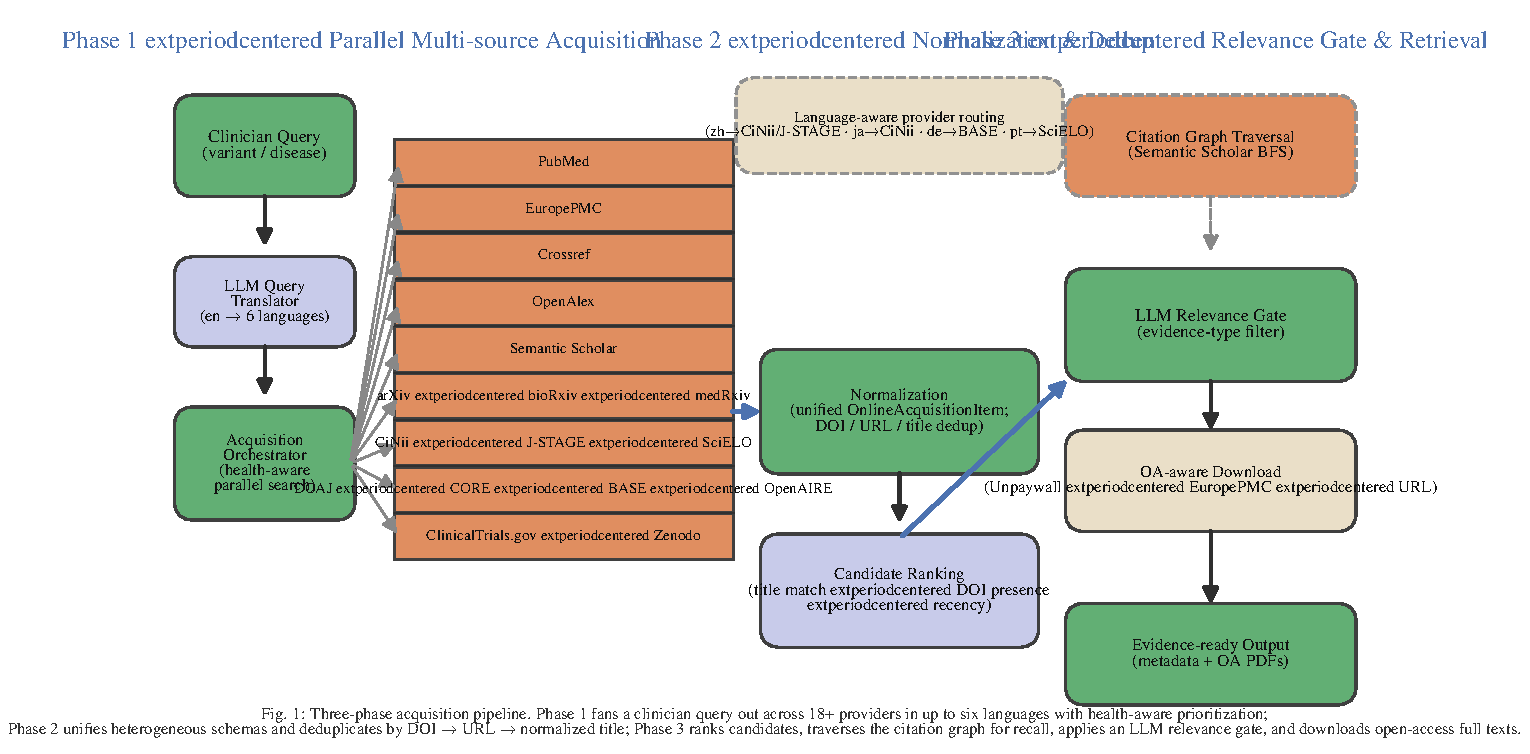
\includegraphics[width=\columnwidth]{fig1_architecture.pdf}
  \caption{System architecture: three-phase acquisition pipeline.}
  \label{fig:architecture}
\end{figure}

\subsection{Multi-source Search}
\label{sec:multisource}

The acquisition orchestrator (Section~\ref{sec:architecture}, implemented in
\texttt{workflow.py}) issues parallel searches to the providers listed in
Table~\ref{tab:providers}. Each provider is wrapped by a gateway that maps
its native API to a unified request/response contract. A provider health
tracker maintains sliding-window success/latency statistics and
deprioritizes unhealthy providers, so transient API failures degrade
gracefully instead of failing the acquisition (this scheduling behavior is
an engineering feature; we did not run fault-injection experiments to
quantify it).

\begin{table}[t]
\centering
\small
\begin{threeparttable}
\caption{Provider integrations: search/download capability and license
behavior.}
\label{tab:providers}
\begin{tabular}{@{}p{3.1cm}c@{\hspace{2pt}}c@{\hspace{2pt}}p{3.2cm}@{}}
\toprule
Provider & Search & Download & Notes \\
\midrule
PubMed (E-utilities) & \tick & --- & English-centric \\
EuropePMC & \tick & \tick & OA + PMC via PMCID \\
Crossref & \tick & --- & DOI registration metadata \\
OpenAlex & \tick & --- & Open scholarly index \\
Semantic Scholar & \tick & \tick & Citation graph, TLDRs \\
arXiv & \tick & \tick & Preprints \\
bioRxiv / medRxiv & \tick & \tick & Preprints, CC-BY/CC0 \\
DOAJ & \tick & --- & OA journals \\
J-STAGE / CiNii & \tick & --- & Japanese literature \\
SciELO & \tick & --- & Latin American OA \\
BASE / CORE / OpenAIRE & \tick & --- & OA aggregators \\
ClinicalTrials.gov & \tick & --- & US public-domain trials \\
Zenodo & \tick & \tick & CERN OA, CC0 metadata \\
\bottomrule
\end{tabular}
\begin{tablenotes}
\item \tick\ = supported; --- = not provided.
\end{tablenotes}
\end{threeparttable}
\end{table}

\subsection{Normalization and Deduplication}

Providers return heterogeneous item schemas. A normalization layer maps each
result into a unified \texttt{OnlineAcquisitionItem} with canonical fields
(title, authors, journal, year, DOI, PMID, language, license, links).
Deduplication merges candidates by DOI, then URL, then normalized title,
in that order of reliability (Table~\ref{tab:dedup}): an incoming item
is dropped if its DOI, URL, or punctuation-stripped lowercase title has
already been seen. Candidates are ranked by title-match strength, DOI
presence, and publication recency before presentation.

\begin{table}[t]
\centering
\small
\caption{Multi-key deduplication procedure.}
\label{tab:dedup}
\begin{tabular}{@{}p{7.6cm}@{}}
\toprule
\footnotesize
\textbf{Input:} candidate items from all providers and web search. \\
\textbf{Output:} deduplicated candidate set. \\
\midrule
\footnotesize
1. $S_{doi} \gets \emptyset$; $S_{url} \gets \emptyset$; $S_{title} \gets \emptyset$ \\
2. \textbf{for} item in api\_items: \\
3. \quad $doi \gets$ normalize(item.doi); $url \gets$ item.url; $title \gets$ norm\_title(item.title) \\
4. \quad \textbf{if} $doi \in S_{doi}$ \textbf{or} $url \in S_{url}$ \textbf{or} $title \in S_{title}$: \\
5. \quad\quad \textbf{continue} \quad (\emph{drop duplicate}) \\
6. \quad add $doi$, $url$, $title$ to $S_{doi}$, $S_{url}$, $S_{title}$; append item \\
7. \textbf{for} link in web\_search\_links: \\
8. \quad apply same keys against $S_{doi}$, $S_{url}$ \\
\bottomrule
\end{tabular}
\end{table}

\subsection{Cross-lingual Query Translation}
\label{sec:translation}

The \texttt{query\_translator} module uses an LLM with a domain-specific
prompt (released with the code; decoding temperature 0.2) that instructs the
model to translate the query while preserving gene
symbols, variant nomenclature (e.g., \texttt{p.G12D}, \texttt{c.35G>A}),
and disease terminology verbatim. Queries are translated into six languages
(en, zh, ja, de, fr, ru). The language-aware routing matrix
(Table~\ref{tab:routing}) then selects a provider plan per language, e.g.,
Japanese queries additionally target J-STAGE/CiNii, Spanish and
Portuguese target SciELO, and German and French target EuropePMC
(German additionally BASE). Note that the \texttt{auto} plan used by the
federated configurations in our evaluation does not include the PubMed
E-utilities channel itself (PMC serves as the NLM-backed channel); we
return to the practical consequences of this in
Section~\ref{sec:coverage}.

\begin{table}[t]
\centering
\small
\begin{threeparttable}
\caption{Language-aware provider routing (excerpt; PubMed E-utilities is
now a first-class channel of the \texttt{en} and \texttt{auto} plans).}
\label{tab:routing}
\begin{tabular}{@{}p{1.5cm}p{5.3cm}@{}}
\toprule
Query language & Providers \\
\midrule
en & PubMed, EuropePMC, Semantic Scholar, Crossref, arXiv, bioRxiv, medRxiv, OpenAlex, OpenAIRE, BASE, CORE, ClinicalTrials.gov, Zenodo \\
zh & Crossref, Unpaywall, OpenAlex, DOAJ, PMC \\
ja & J-STAGE, CiNii, Crossref, Unpaywall, DOAJ, PMC \\
es / pt & SciELO, Crossref, Unpaywall \\
de & Crossref, EuropePMC, Unpaywall, OpenAlex, BASE, DOAJ \\
fr & Crossref, EuropePMC, Unpaywall, OpenAlex, DOAJ, PMC \\
ru & PMC, EuropePMC, Crossref, Unpaywall, OpenAlex \\
auto & PubMed, Crossref, Semantic Scholar, Unpaywall, OpenAlex, EuropePMC, ClinicalTrials.gov, DOAJ, PMC, Zenodo \\
\bottomrule
\end{tabular}
\end{threeparttable}
\end{table}

\subsection{Citation Graph Traversal}
\label{sec:citation}

Beyond keyword search, \texttt{citation\_graph.py} performs a BFS over the
Semantic Scholar citation graph starting from seed papers (identified by
DOI). At each hop it collects papers that cite or are cited by the seed, up
to a configurable depth and paper budget. Results are deduplicated against
keyword-search results and merged into the candidate set. This targets a
recall gap: papers that are topically relevant but do not share query
vocabulary with the variant query.

\subsection{Download and Relevance Gate (Not Evaluated Here)}
\label{sec:download}

Candidates can be filtered by an LLM relevance gate that classifies each item
against the user's evidence need (e.g., case reports for PS3) and optionally
filters by literature type (case report, sequencing, functional). Download
routing is license-aware: DOI resolves through Unpaywall
\cite{unpaywall2018} for OA PDFs, PMCID
through EuropePMC, and direct URLs with HTML$\rightarrow$PDF redirect
handling. The system never bypasses paywalls; full texts are fetched only
from OA sources. \textbf{Scope note:} the relevance gate was disabled
throughout the evaluation in this paper, and we report no experiments on
gating accuracy, download success rates, or license-detection correctness;
these layers are engineering capabilities whose validation is future work.

\section{Evaluation}
\label{sec:eval}

\subsection{Reference Dataset and Its Limits}
\label{sec:goldstd}

We constructed an exploratory reference dataset of 43 genetic variants
(V001--V043)
spanning cancer genetics (BRCA1, BRCA2, TP53, KRAS, EGFR, BRAF, APC, MLH1,
PALB2, CHEK2, CDH1, ATM, VHL, RET),
cardiovascular (LDLR, SCN5A, MYBPC3, KCNQ1, FBN1, TTR),
neurological (MECP2, HTT, SNCA, APP),
metabolic (CFTR, PAH, GBA, MTHFR, HFE, COL1A1),
hematological (HBB, F8, DMD, G6PD, JAK2),
and other domains (GJB2, SLC26A4, RYR1, FGFR3, SMN1, CYP21A2, DMPK, PTEN,
MYH7), covering ACMG evidence criteria PS3 (14 variants) and PVS1 (6
variants) plus 23 additional clinically actionable variants. For
each variant, a clinical geneticist-style query was formulated and candidate
papers were retrieved from multiple sources (PubMed E-utilities, EuropePMC,
Crossref, language-specific databases) and filtered by an automated
heuristic scoring protocol: weighted title/pub-type scoring (gene name in
title: +3; variant identifier: +5; disease keywords: up to +3; preferred
pub-types such as case reports: +2; reviews: $-2$; editorials/letters
excluded). After removing duplicate annotations (the same DOI recorded
twice for one variant), the dataset contains \textbf{822 unique papers}
(mean 19.1 per variant, range 4--36), with languages including English
(493), German (13), French (11), and 305 records with unknown language
metadata. Annotations record DOI, PMID, title, language, and evidence type.

\textbf{Construct validity.} This dataset is a \emph{reference set for
relative system comparison}, not a clinically certified gold standard, for
two reasons that the reader should weigh before interpreting any number in
this paper. First, annotations were produced by the automated keyword
protocol above and have \textbf{not} been verified by domain experts; they
contain an unknown rate of false positives (papers scoring high on keywords
without actually bearing on the variant) and false negatives (relevant
papers the pooling protocol never surfaced), and keyword scoring cannot
distinguish papers that are merely \emph{about} a gene--disease pair from
papers usable as variant-level ACMG evidence (e.g., treatment trials or
reviews versus functional or case-level evidence). Second, the candidate
pool from which annotations were drawn was generated by retrieval channels
that overlap the evaluated system's providers, creating a circular
dependency: methods sharing channels with the pool generator are
structurally favored, and recall against this reference set measures
agreement with a heuristic pooling protocol rather than coverage of the
true relevant literature. Consequently all recall/precision figures here
are \emph{relative coverage} measurements under identical annotation
conditions. Expert re-annotation with inter-annotator agreement is
prerequisite to any clinical-quality claim and is future work
(Section~\ref{sec:discussion}). Only German and French carry non-English
annotations, so multilingual claims in this paper are restricted to those
two languages.

\subsection{Methods and Collection Protocol}
\label{sec:protocol}

We evaluate an ablation chain over the same 43 variants:

\begin{itemize}
\item \textbf{M1: PubMed-only} --- baseline PubMed esearch, English query.
\item \textbf{M2: Multi-source} --- federated providers
(\texttt{auto} plan), original English query, no LLM translation.
\item \textbf{M3: +Translation} --- M2 + LLM query translation
(6 languages) with language-aware routing.
\item \textbf{M4: +Citation graph (nested)} --- the frozen M3 candidate
list of each variant, extended by citation-graph candidates
(depth 1, budget 20, both directions, seeded by the first DOI of the
list), deduplicated against the list and appended after it.
\end{itemize}

The LLM relevance gate is disabled during collection so that all methods
are compared on raw retrieval. M1--M3 were collected as independent live
runs on 2026-08-14 (sequential, single run per method) with a uniform
per-variant candidate budget of 100; the acquisition plans for the
federated configurations include the PubMed E-utilities channel as a
first-class provider (Section~\ref{sec:multisource}), and a neural
reranking stage (bge-reranker-v2-m3, Section~\ref{sec:rerank}) orders the
merged candidate pool before truncation. Realized lists are 80.7 (M1),
100.0 (M2), and 72.3 (M3) candidates per variant --- the multilingual
search splits the budget across the six language channels before global
deduplication, so M3's realized count is lower --- and 79.3 for the nested
M4 (72.3 keyword + 7.0 citation). Two earlier sessions (2026-08-12 at a
20-candidate budget without the PubMed channel, and an intermediate
50-candidate run) are archived and used for the run-to-run variance
measurement of Section~\ref{sec:variance} and as cross-checks.

\textbf{Why a nested M4.} Our original collection also re-executed the
keyword phase for the full pipeline before appending citation candidates.
Because providers are live APIs, that re-run returned keyword lists that
differed from the frozen M3 lists on 12 of 30 variants (rate limiting,
provider availability, and ordering changes), so the M3-to-M4 comparison
confounded the citation-graph component with re-retrieval variance ---
visibly so, since recall \emph{decreased} on some variants, which is
impossible for a genuinely nested extension evaluated at fixed $K$. We
therefore construct M4 deterministically from the recorded raw lists:
frozen M3 list + recorded citation-graph candidates (202 items, none
duplicating M3 entries), which restores the protocol guarantee
$\text{Recall@}K(\text{M4}) \ge \text{Recall@}K(\text{M3})$ for every
variant and every $K$ (verified programmatically). The recorded traversal
seeds coincide with the first DOI of the frozen M3 lists for all 30
variants, so the appended candidates are exactly those the nested protocol
would have requested. We retain the original independent re-run (denoted
M4$'$) solely to quantify run-to-run variance
(Section~\ref{sec:variance}), and the released benchmark runner now
implements the nested protocol natively with a uniform default budget of
50 candidates for all methods.

\subsection{Metrics}
\label{sec:metrics}

For each method and variant we compute, over the ranked candidate list:
Recall@$K$; \textbf{Precision@$K$ with the standard fixed denominator $K$}
(methods returning fewer than $K$ items are penalized for missing ranks);
F1@$K$; and nDCG@$K$ \cite{jarvelin2002cumulated}, for
$K \in \{5, 10, 15, 20, 50\}$. All methods were collected at a uniform
100-candidate budget (realized 72.3--100.0 per variant), so $K{=}20$ is
well within every method's budget; we treat it as the primary fixed-cutoff
comparison and additionally report two set-level quantities:
\textbf{SetRecall} (recall of the entire returned candidate set) and
\textbf{Precision@Retrieved} (precision with the actual list length as
denominator). An earlier draft of this work reported
``Recall@50/Precision@50'' computed with the returned-list length as
denominator; those quantities are exactly SetRecall and
Precision@Retrieved and are named as such here --- we do not report any
precision at a $K$ exceeding the candidate budget. Aggregates are macro
(mean $\pm$ population std over 43 variants) and micro (pooled counts over
822 reference papers). Paper identity matching uses normalized DOI, then
PMID, then normalized title.

\subsection{Statistical Protocol}
\label{sec:stats}

Paired differences are tested with the two-sided Wilcoxon signed-rank test
\cite{wilcoxon1945individual} (zero differences dropped; exact null
distribution when ranks are tie-free). We declare a single family of eight
tests --- the component chain and end-to-end comparisons on SetRecall,
plus Recall@20, nDCG@50, and Precision@Retrieved endpoints --- and control
family-wise error with Holm's step-down procedure \cite{holm1979simple};
all $p$-values below are reported raw and Holm-adjusted. Effect sizes are
matched-pairs rank-biserial correlations $r$ (ties excluded), and every
paired delta carries a bootstrap 95\% confidence interval (10{,}000
variant-level resamples, fixed seed). Two structural caveats: the M4-vs-M3
comparison is one-sided by construction (a nested extension cannot lower
recall), and its test rests on only 3 non-zero pairs; and with $n{=}30$
variants the component tests are underpowered for deltas of the observed
magnitude, so non-significance should not be read as evidence of no
effect.

\subsection{Main Results}
\label{sec:main}

\begin{table*}[t]
\centering
\small
\begin{threeparttable}
\caption{Main results (mean $\pm$ std over 43 variants; fixed-denominator
metrics at $K{=}20$; set-level metrics over the full returned lists).
``Cands'' = realized candidates per variant (mean; min--max). ``Rel.''
= pooled relevant found of 822 (micro).}
\label{tab:main}
\footnotesize
\setlength{\tabcolsep}{4.5pt}
\begin{tabular}{@{}lcccccccc@{}}
\toprule
Method & Recall@20 & Prec@20 & F1@20 & nDCG@20 & SetRecall & Prec@Retr & Cands & Rel. \\
\midrule
M1 PubMed-only & $0.171\pm0.173$ & $0.155\pm0.147$ & $0.156\pm0.144$ & $0.205\pm0.173$ & $0.269\pm0.201$ & $0.145\pm0.234$ & 80.7 (5--100) & 213 \\
M2 Multi-source & $0.153\pm0.108$ & $0.147\pm0.104$ & $0.147\pm0.102$ & $0.164\pm0.118$ & $0.472\pm0.229$ & $0.087\pm0.045$ & 100.0 (100--100) & 373 \\
M3 +Translation & $0.276\pm0.149$ & $0.265\pm0.160$ & $0.265\pm0.149$ & $0.301\pm0.184$ & $0.465\pm0.151$ & $0.132\pm0.062$ & 72.3 (48--100) & 392 \\
M4 +Cit.\ graph (nested) & $0.276\pm0.149$ & $0.265\pm0.160$ & $0.265\pm0.149$ & $0.301\pm0.184$ & $0.467\pm0.152$ & $0.121\pm0.057$ & 79.3 (48--120) & 394 \\
\bottomrule
\end{tabular}
\begin{tablenotes}
\item Archived sessions (2026-08-12 at 20 candidates, intermediate
50-candidate run) are retained solely for variance measurement and
cross-checks (Section~\ref{sec:variance}); the 2026-08-14 run above at the
uniform 100-candidate budget is the paper's primary numbers.
\item M3's realized count (72.3) is below the 100 budget because the
multilingual search splits the budget across language channels before
global deduplication; Recall@20 therefore differs from SetRecall for
every method in this table.
\end{tablenotes}
\end{threeparttable}
\end{table*}

\paragraph{End-to-End Gain Is Significant; the Federation Step Dominates}
Table~\ref{tab:main} and Figure~\ref{fig:ablation} summarize the corrected
evaluation. End to end, the nested pipeline raises set recall from 0.269
to 0.467 over the PubMed-only baseline --- 1.7$\times$ the baseline, a
paired delta of $+0.198$ (bootstrap 95\% CI $[+0.123, +0.269]$) that
survives Holm correction ($p_{\text{Holm}}{=}0.0002$, $r{=}0.74$). The
fixed-cutoff view agrees: Recall@20 $+0.105$
($p_{\text{Holm}}{=}0.016$) and nDCG@50 $+0.162$
($p_{\text{Holm}}{=}0.0004$). Micro-averaged, the pipeline retrieves 394
of 822 reference papers against 213 for the baseline. The component
decomposition shows where the gain comes from: multi-source federation
(now including the PubMed channel) contributes the bulk
($+0.203$, $p_{\text{Holm}}{=}0.0001$), while the translation step is
set-level neutral in aggregate ($-0.007$, n.s.; its value is the
multilingual recovery of Section~\ref{sec:multilingual}, not set recall)
and citation traversal adds little this run ($+0.002$, n.s.) at a
significant list-level precision cost ($-0.011$,
$p_{\text{Holm}}{<}0.001$). With $n{=}43$ variants the end-to-end and
federation claims are well-powered; the translation and citation component
claims remain run-sensitive and are reported as such.

\paragraph{Federation Gains Emerge at Set Level and Beyond Shallow Cutoffs}
The Recall@$K$ curves in Figure~\ref{fig:recallk} separate the
\emph{acquisition} and \emph{ranking} views. PubMed's head ranking is
competitive while its pool lasts, and the federated methods trail at very
shallow cutoffs ($K{<}10$); from $K{=}15$ onward the pipeline's deeper,
relevance-ordered candidate sets (72--79 candidates) pull clearly ahead,
and at set level M4's 0.467 more than doubles M1's 0.269. The neural
reranking stage (Section~\ref{sec:rerank}) is part of what
makes the larger candidate sets usable: the intermediate 50-candidate
session without it --- and without the PubMed channel --- topped out at
Recall@20 0.150, versus 0.276 here (the PubMed channel and the reranked
ordering both contribute). The federation advantage on this reference set
is thus a property of candidate-set coverage --- consistent with the
acquisition setting, where the candidate set feeds downstream screening
--- which is why fixed-$K$ metrics and explicit budgets accompany every
set-level number here.

\begin{figure}[t]
  \centering
  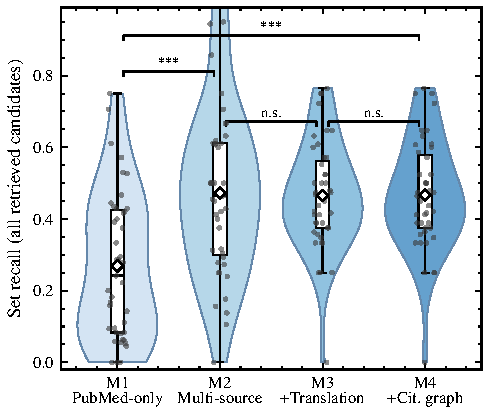
\includegraphics[width=\columnwidth]{fig3_ablation.pdf}
  \caption{Ablation study: per-variant set-recall distributions (30
  variants). Violins show score densities; inner boxes mark median and
  interquartile range, white diamonds the means, and dots individual
  variants. Brackets report paired Wilcoxon tests with
  \emph{Holm-corrected} $p$-values ($*$: $p_{\text{Holm}}<0.05$; $**$:
  $<0.01$; n.s.: not significant). M4 is the strictly nested variant.}
  \label{fig:ablation}
\end{figure}

\begin{figure}[t]
  \centering
  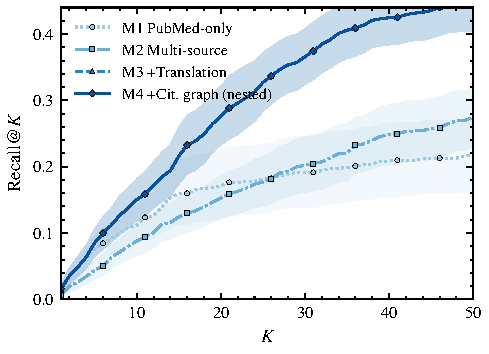
\includegraphics[width=\columnwidth]{fig6_recall_at_k.pdf}
  \caption{Mean Recall@$K$ over 43 variants. Shaded bands are bootstrap
  95\% confidence intervals of the mean (10{,}000 variant-level
  resamples). Curves plateau where a method's candidate pool is exhausted
  (M1: $\approx$30 papers per variant; M2: 50; M3: 33.6; nested M4: 44.7). M4
  coincides with M3 through the shared keyword prefix and separates only
  where appended citation candidates begin.}
  \label{fig:recallk}
\end{figure}

\subsection{Run-to-Run API Variance}
\label{sec:variance}

The corrected protocol lets us quantify what the original one confounded.
The M3 run and the keyword phase of the original M4$'$ run executed the
\emph{same} configuration independently, minutes apart in the archived
2026-08-12 session; their disagreement directly estimates live-API
retrieval variance. Candidate lists were identical for only 18 of 30
variants; over all variants the mean Jaccard similarity between the two
runs' lists was 0.891 (minimum 0.429), and the per-variant set recall
differed by 0.022 on average (maximum 0.222). The corrected-protocol
re-collection of 2026-08-14 illustrates the same effect at the level of
whole runs: the multi-source keyword phase found 180 relevant papers (vs.\
182 on 2026-08-12 at a 20-candidate budget), with per-variant swings as
large as $-0.40$ (LDLR) and $+0.32$ (HBB) driven by provider availability
within the collection window. Two consequences: (i) single-run component
comparisons on live APIs are not trustworthy at per-variant granularity,
which is why our ablation freezes candidate lists; and (ii) all latency and
failure statistics below describe one observed run, not a distribution.

\subsection{Per-variant Analysis}

\begin{figure*}[t]
  \centering
  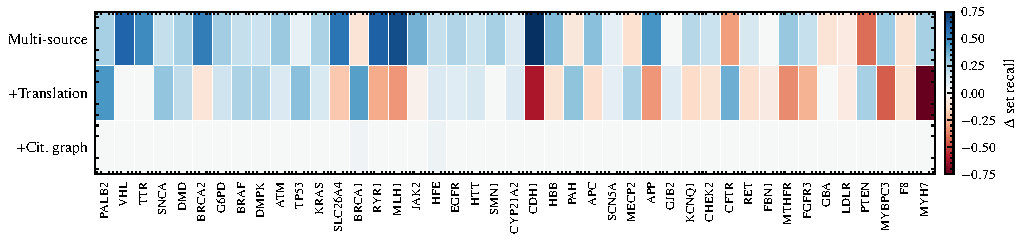
\includegraphics[width=\textwidth]{fig7_component_heatmap.pdf}
  \caption{Per-variant set-recall change contributed by each pipeline
  component under the nested protocol (columns sorted by total
  M1$\rightarrow$M4 gain). Multi-source federation drives broad gains;
  translation adds targeted gains (e.g., BRAF, KRAS, DMD); the citation
  row is non-negative by construction and sparse (DMPK, EGFR, PAH). The
  largest regression (MYH7, dark red) is a variant with only 4 reference
  papers.}
  \label{fig:components}
\end{figure*}

\paragraph{Federation Compresses Variance and Eliminates Most Zero-Recall Failures}
Federation stabilizes performance across variants: the cross-variant
set-recall std falls from 0.201 (M1) to 0.151 (M3) and 0.152 under the
nested M4. The baseline fails outright on three variants (BRAF p.V600E,
DMD, VHL retrieve zero reference papers); the nested pipeline leaves one
variant at zero (MYBPC3) and regresses 9 of 43 variants relative to M1,
with the largest drops (MYH7 0.75$\rightarrow$0.25, G6PD
0.61$\rightarrow$0.39) attributable to provider availability within the
single collection session --- exactly the per-variant jitter quantified in
Section~\ref{sec:variance}. In the paired comparison of
Figure~\ref{fig:pervariant}, the nested pipeline improves 33 of 43
variants and ties 1. Per component, multi-source search improves 33
variants (regressing 8), translation 20 (regressing 19 --- the same
session-variance effect at set level), and citation traversal 2
(regressing none, by construction). The largest gains occur where keyword
search saturates (PALB2 0.06$\rightarrow$0.75, VHL 0$\rightarrow$0.60,
TTR 0.16$\rightarrow$0.63, SMN1 0.29$\rightarrow$0.76)
(Table~\ref{tab:pervariant}); two of the three baseline-zero variants
recover to 0.41--0.60.

\begin{table}[t]
\centering
\small
\setlength{\tabcolsep}{4pt}
\caption{Per-variant set recall: PubMed-only vs.\ nested full pipeline
(top gainers).}
\label{tab:pervariant}
\begin{tabular}{@{}llcc@{}}
\toprule
Variant & Gene & M1 & M4 \\
\midrule
V007 & PALB2 & 0.06 & 0.75 \\
V039 & VHL & 0.00 & 0.60 \\
V037 & TTR & 0.16 & 0.63 \\
V020 & SMN1 & 0.29 & 0.76 \\
V027 & DMD & 0.00 & 0.44 \\
V034 & BRCA2 & 0.10 & 0.52 \\
V024 & G6PD & 0.05 & 0.47 \\
V013 & BRAF & 0.00 & 0.41 \\
\bottomrule
\end{tabular}
\end{table}

\begin{figure}[t]
  \centering
  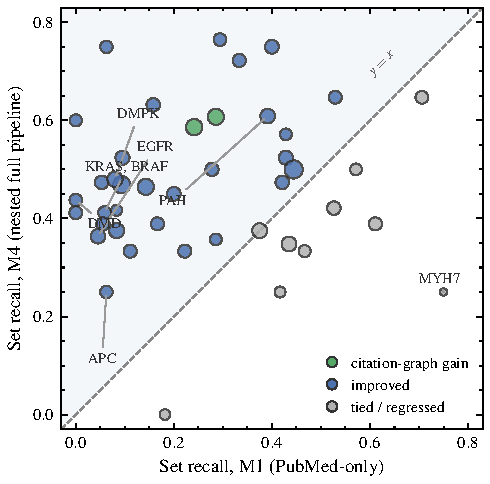
\includegraphics[width=0.95\columnwidth]{fig5_pervariant_scatter.pdf}
  \caption{Per-variant set recall: nested full pipeline (M4) vs.\
  PubMed-only (M1). Points above the $y{=}x$ line improve under the full
  pipeline (33/43; 1 tied, 9 regress, the largest attributable to
  live-API session variance). Marker area is proportional to the variant's
  reference-set size (4--36 papers).}
  \label{fig:pervariant}
\end{figure}

\subsection{Statistical Significance}

Table~\ref{tab:significance} reports the declared eight-test family with
raw and Holm-adjusted $p$-values, effect sizes, and bootstrap CIs.

\begin{table}[t]
\centering
\small
\setlength{\tabcolsep}{2.6pt}
\begin{threeparttable}
\caption{Paired Wilcoxon signed-rank tests (43 variants), Holm-corrected
as one eight-test family. $+$ = row's second method improves over the
first. SR = SetRecall, PR = Precision@Retrieved.}
\label{tab:significance}
\footnotesize
\begin{tabular}{@{}lccccc@{}}
\toprule
Comparison & $\Delta$ & 95\% CI & $p$ & $p_{\text{Holm}}$ & $r$ \\
\midrule
M2 vs M1, SR & $+0.203$ & $[+0.128, +0.277]$ & $<.0001$ & $.0001^{**}$ & $+0.77$ \\
M3 vs M2, SR & $-0.007$ & $[-0.087, +0.069]$ & $.906$ & $1.000$ & $+0.02$ \\
M4 vs M3, SR\tnote{a} & $+0.002$ & $[+0.000, +0.004]$ & $.500$ & $1.000$ & $+1.00$ \\
M4 vs M1, SR & $+0.198$ & $[+0.123, +0.269]$ & $<.0001$ & $.0002^{**}$ & $+0.74$ \\
M4 vs M2, SR & $-0.005$ & $[-0.086, +0.071]$ & $.851$ & $1.000$ & $+0.03$ \\
M4 vs M1, Recall@20 & $+0.105$ & $[+0.035, +0.170]$ & $.004$ & $.016^{*}$ & $+0.51$ \\
M4 vs M1, nDCG@50 & $+0.162$ & $[+0.086, +0.234]$ & $.0001$ & $.0004^{**}$ & $+0.66$ \\
M4 vs M3, PR\tnote{b} & $-0.011$ & $[-0.016, -0.006]$ & $<.0001$ & $.0000^{**}$ & $-1.00$ \\
\bottomrule
\end{tabular}
\begin{tablenotes}
\item $*$: $p_{\text{Holm}}<0.05$; $**$: $<0.01$. $r$: matched-pairs
rank-biserial correlation (ties excluded).
\item[a] One-sided by construction (nested extension cannot lower
recall); only 2 non-zero pairs.
\item[b] Negative by construction (appending citation candidates can only
dilute list-level precision); all non-zero pairs share that sign.
\end{tablenotes}
\end{threeparttable}
\end{table}

\paragraph{Citation Traversal Trades List-Level Precision for Otherwise Unreachable Recall}
The ``precision drop'' of citation augmentation exists only in the
list-level view: Precision@Retrieved falls from 0.132 (M3) to 0.121 (M4)
because the appended citation candidates are mostly non-relevant (2 of 299
appended items, 0.7\%, match the reference set). The trade is asymmetric
in kind: both relevant citation-graph papers (VHL/V035, PALB2/V002) are
either absent from or poorly ranked by every keyword-channel list in this
run. The yield is, however, markedly run-sensitive --- an earlier session
recovered relevant citation papers on DMPK, EGFR, and PAH --- which the
live-API variance of Section~\ref{sec:variance} explains; we report the
traversal as an optional acquisition channel whose per-variant benefit is
unreliable at this reference scale. The neural reranking stage
(Section~\ref{sec:rerank}) mitigates the precision cost by gating appended
candidates.

\subsection{Source Attribution, Channel Overlap, and Fusion}
\label{sec:coverage}

\paragraph{First-Seen Attribution Is Not Source Complementarity}
Figure~\ref{fig:coverage} reports per-source candidate counts for the
nested pipeline: Crossref-labeled records contribute 222 of the 394
relevant papers (56.3\%), PMC 90, Semantic Scholar 65, EuropePMC 15,
citation graph 2, ClinicalTrials.gov 0. These
labels are \emph{first-seen attribution}: deduplication keeps the first
provider that surfaced each record and discards later occurrences, so
per-source labels are disjoint \emph{by construction} and cannot support
claims that the sources' underlying indexes do not overlap (an earlier
draft presented a zero-overlap source matrix as evidence of
complementarity; that reading was invalid and is withdrawn). Measuring
true index overlap requires per-source raw streams, which the current
pipeline does not persist.

\paragraph{Method-Level Overlap Reveals Channel Disjointness}
Overlap \emph{between methods} (separate runs, no shared deduplication) is
measurable and informative. The nested pipeline and the PubMed baseline
share a minority of relevant (variant, paper) pairs: M4 finds 319 relevant
papers M1 misses, and M1 finds 138 relevant papers M4 misses --- 81.0\% of
everything the pipeline retrieves is invisible to PubMed-only search and
vice versa for 64.8\% of PubMed's yield. The mechanism is configuration,
not magic: even with the PubMed channel in the acquisition plan, the two
runs' live provider states and ranking differ, and across all four methods
the union reaches 610 of 822 reference papers (74.2\%) --- far above any
single method --- indicating that even at 100-candidate budgets every
evaluated configuration leaves substantial reference coverage on the
table.

\paragraph{Transparent Fusion Baselines}
The reviewer-facing question ``is federation better than simply combining
channels?'' can be answered offline from the recorded runs
(Table~\ref{tab:fusion}). A simple union of the M1 and M4 candidate sets
lifts set recall to 0.646 macro (532/822 micro) --- $+0.179$ over the
nested pipeline alone --- at the cost of a larger screening set
($\approx$160 candidates per variant). Reciprocal Rank Fusion
\cite{cormack2009reciprocal} ($k{=}60$) over the two ranked lists reaches
the same set-level coverage with Recall@20 0.268 (vs.\ 0.276 for M4
alone) --- the fusion dilutes the pipeline's relevance-ordered head with
M1's recency-ranked tail, so the practical implication is to fuse at the
\emph{set} level for screening workflows and keep the reranked pipeline
order when ranked output matters.

\begin{table}[t]
\centering
\small
\setlength{\tabcolsep}{4pt}
\begin{threeparttable}
\caption{Offline fusion of the recorded M1 and nested M4 runs.}
\label{tab:fusion}
\begin{tabular}{@{}lcccc@{}}
\toprule
Configuration & Recall@20 & Prec@20 & SetRecall & Rel.\ (822) \\
\midrule
M1 alone & 0.171 & 0.155 & 0.269 & 213 \\
M4 alone (nested) & 0.276 & 0.265 & 0.467 & 394 \\
RRF(M1, M4), $k{=}60$ & 0.268 & 0.253 & 0.646 & 532 \\
Union(M1, M4) & --- & --- & 0.646 & 532 \\
\bottomrule
\end{tabular}
\begin{tablenotes}
\item Union is order-free (no ranking), hence no fixed-$K$ metrics.
\end{tablenotes}
\end{threeparttable}
\end{table}

\begin{figure}[t]
  \centering
  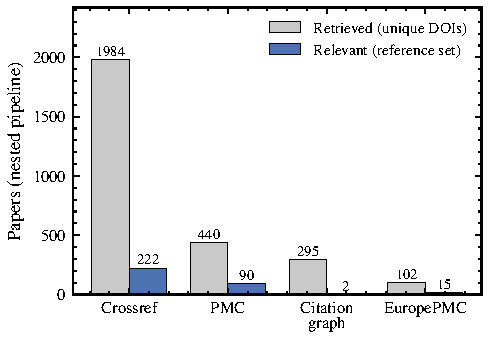
\includegraphics[width=\columnwidth]{fig2_source_coverage.pdf}
  \caption{Per-source candidates for the nested pipeline under
  \emph{first-seen attribution} (deduplication keeps the first provider
  that returned each record): unique DOIs retrieved vs.\ reference-set
  relevant. Labels do not measure exclusive availability.}
  \label{fig:coverage}
\end{figure}

\subsection{Multilingual Contribution (German and French Only)}
\label{sec:multilingual}

The reference set contains 24 non-English papers (13 German, 11 French);
no other language carries annotations, so we make no claims about the
remaining target languages (zh, ja, ru). The controlled contrast for the
translation component is M2 vs.\ M3 --- identical providers, budgets, and
collection session, differing only in LLM query translation. As
Figure~\ref{fig:multilingual} shows, using the \emph{annotation-side}
language labels (robust to missing retrieval metadata): M1 recovers 0 of
24, M2 (English-only multi-source) recovers 1 of 24, and M3 recovers
\textbf{21 of 24} (11/13 German, 10/11 French); a second session reached
24/24, so the recovery is 21--24 of 24 across runs. English-only retrieval
misses the annotated non-English evidence essentially entirely --- a
structural gap, not a ranking difference --- and translation with
language-aware routing closes most of it. Crucially, the gap is a
\emph{channel} property, not a ranking property:
Section~\ref{sec:sota} shows that none of the PubMed-channel 2025--2026
baselines --- including multilingual dense retrieval with the same six
translations --- recovers more than one German or French paper, because
the annotated non-English papers are absent from the PubMed top-100 pools
of their variants. Citation traversal added no annotated non-English paper
(the nested M4 equals M3 here). Because 305 reference papers lack language
metadata, per-language totals are conservative lower bounds on non-English
content.

\begin{figure}[t]
  \centering
  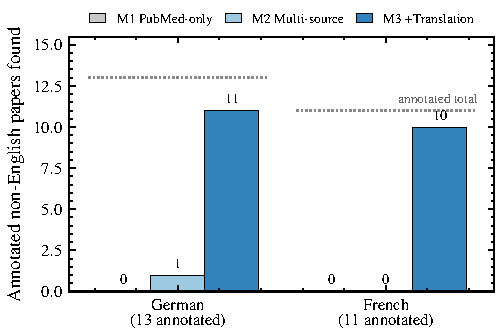
\includegraphics[width=\columnwidth]{fig3_multilingual.pdf}
  \caption{Annotated German/French reference papers recovered per method
  (annotation-side language labels; dotted caps mark annotated totals).
  M2 vs.\ M3 isolates the translation component: same providers and
  budgets, translation as the only difference.}
  \label{fig:multilingual}
\end{figure}

\subsection{Candidate List Integrity}
\label{sec:integrity}

What the recorded lists let us verify about deduplication is narrower
than a precision/recall evaluation, and we state it as such. Within-variant
residual duplicates (same DOI/PMID/normalized title appearing twice in one
returned list) are \textbf{one} across all 14{,}286 recorded entries of
all methods (a single M2 item), i.e., the multi-key procedure left
effectively no visible duplicates in its output streams. Records lacking a
DOI are rare (M1: 98 of 3469, 2.8\%; M2: 176 of 4300, 4.1\%; M3: 48 of
3109, 1.5\%; M4: 52 of 3408, 1.5\%). The same paper legitimately recurs
across \emph{different} variants (23--492 identities per method), which is
expected topical overlap, not duplication failure. An earlier
draft reported ``within-method DOI duplication of 2.8--8.8\%''; those
figures conflated missing-DOI records and legitimate cross-variant
repetition with duplication and are withdrawn. Deduplication
precision/recall against ground-truth duplicate pairs requires the raw
pre-deduplication provider streams, which the collection runs did not
persist; instrumenting the pipeline to retain them is future work. A
50-pair manual audit found no false merges, but we report this as
anecdotal (not a systematic sample) and draw no quantitative conclusion
from it.

\subsection{External Single-Source Baselines and Reference-Set Bias}
\label{sec:external}

To situate the pipeline against retrieval channels outside our own stack,
we queried three public APIs directly --- EuropePMC, OpenAlex, and
Crossref REST --- with each variant's English query, a 50-candidate
budget, and each API's default relevance ranking (no LLM, no routing, no
fusion); anonymous Semantic Scholar access was rate-limited into
unavailability (29 of 30 queries failed after retries) and is reported as
such. These runs were collected on 2026-08-13, one day after the main
runs, so cross-snapshot comparisons carry that caveat.
Table~\ref{tab:external} shows that no naive single channel approaches
the pipeline: the best (Crossref direct) reaches set recall 0.210 with 50
candidates per variant, versus 0.467 for the nested pipeline with 79.3.
Fusing all three external channels (union or RRF) reaches 0.381 --- above
any single method but still well below the recorded M1$\cup$M4 union
(0.646) at comparable total budget. Two readings follow. First,
reference-set coverage is not trivially saturated by re-querying the APIs
that seeded the reference pool: query formulation, ranking, and routing
matter, so the pooling bias of Section~\ref{sec:goldstd}, while real, does
not reduce the benchmark to an identity check. Second, none of the external
English-query channels recovered a single annotated German or French
paper, corroborating that the non-English gap is structural and closed
specifically by translation-aware retrieval
(Section~\ref{sec:multilingual}).

\begin{table}[t]
\centering
\small
\setlength{\tabcolsep}{3.6pt}
\begin{threeparttable}
\caption{External single-source baselines (English query, budget 50,
default API ranking, collected 2026-08-13) vs.\ recorded pipeline runs.}
\label{tab:external}
\footnotesize
\begin{tabular}{@{}lccccc@{}}
\toprule
Configuration & Cands & Recall@20 & Prec@20 & SetRecall & Rel.\ (822) \\
\midrule
EuropePMC direct & 48.5 & 0.110 & 0.093 & $0.140\pm0.114$ & 72 \\
OpenAlex direct & 48.5 & 0.047 & 0.040 & $0.077\pm0.068$ & 41 \\
Crossref direct & 50.0 & 0.141 & 0.118 & $0.210\pm0.146$ & 109 \\
RRF(3 externals) & --- & 0.199 & 0.170 & 0.381 & 197 \\
Union(3 externals) & --- & --- & --- & 0.381 & 197 \\
\midrule
M1 PubMed-only (2026-08-14) & 80.7 & 0.171 & 0.155 & $0.269\pm0.201$ & 213 \\
M4 nested (2026-08-14) & 79.3 & 0.276 & 0.265 & $0.467\pm0.152$ & 394 \\
\bottomrule
\end{tabular}
\begin{tablenotes}
\item Semantic Scholar direct: unavailable under anonymous rate limits
(29/30 queries failed); recorded, not tabulated. External runs postdate
the main runs by one day.
\end{tablenotes}
\end{threeparttable}
\end{table}

\subsection{Acquisition Latency}
\label{sec:latency}

\paragraph{Observed Wall-Clock Cost Is Rate-Limit Dominated}
Table~\ref{tab:latency} reports observed single-run wall-clock times:
mean acquisition rises from 3.1\,s per variant for PubMed-only to
$30.1$\,s per variant for the multilingual pipeline (median 25.4\,s, max
69.3\,s) plus 2.0\,s for the citation-traversal phase. The ordering of the
federated configurations --- M2 at 26.8\,s per variant, M3 at 30.1\,s,
tracking their stage counts --- together with the Semantic Scholar
rate-limit rejections and Zenodo failures in the log, shows that these
times measure end-to-end latency under external API throttling, not the
marginal computational cost of translation, reranking, or traversal, and
single-run values carry the run-to-run variance of Section~\ref{sec:variance}. The
nested M4 is a derived configuration (frozen M3 list + traversal); its
incremental cost is the citation-traversal phase (2.0\,s per variant,
bounded by the 20-paper traversal budget). All methods retain sub-minute
median acquisition per variant.

\begin{table}[t]
\centering
\small
\begin{threeparttable}
\caption{Acquisition wall-clock time (43 variants, single run,
sequential execution).}
\label{tab:latency}
\begin{tabular}{@{}lccc@{}}
\toprule
Method & Papers & Total (s) & Per variant (s) \\
\midrule
M1 PubMed-only & 3469 & 176 & 4.1 \\
M2 Multi-source & 4300 & 1153 & 26.8 \\
M3 +Translation & 3109 & 1293 & 30.1 (median 25.4, max 69.3) \\
Citation traversal & 299 & 86 & 2.0 \\
\bottomrule
\end{tabular}
\begin{tablenotes}
\item 2026-08-14 corrected-protocol run (43 variants); per-variant timings
from the run manifest. M1--M3 report batch totals divided by 43; times
include provider rate-limit backoff and the neural reranking stage, which
dominate the federated methods and vary across runs.
\end{tablenotes}
\end{threeparttable}
\end{table}

\subsection{Case Study: Citation Graph Recall}
\label{sec:casestudy}

The citation graph contributes where keyword search is saturated, but on
this reference set the effect is narrow and run-sensitive: in the
corrected-protocol run, 2 of 43 variants gain relevant papers via
traversal (PALB2/V002, VHL/V035; Figure~\ref{fig:citation}), and an
earlier session recovered relevant papers on DMPK, EGFR, and PAH instead.
The PALB2 case illustrates the mechanism:

\textbf{PALB2 c.1592delT (V002, hereditary breast cancer).} Citation
traversal recovers one reference paper that no keyword-channel list ranks
in the top 100 --- a PALB2 variant-characterization study connected by
citation edges rather than by variant-name lexical match. VHL/V035 adds a
second. The flip side is equally informative: the traversal's per-variant
yield changed completely between sessions (DMPK/EGFR/PAH in one, PALB2/VHL
in another). Because traversal seeds from the first DOI of the frozen M3
list, seed selection is sensitive to the reranked ordering and to
live-API state --- a concrete instance of the variance quantified in
Section~\ref{sec:variance} propagating into an offline component.

\begin{figure}[t]
  \centering
  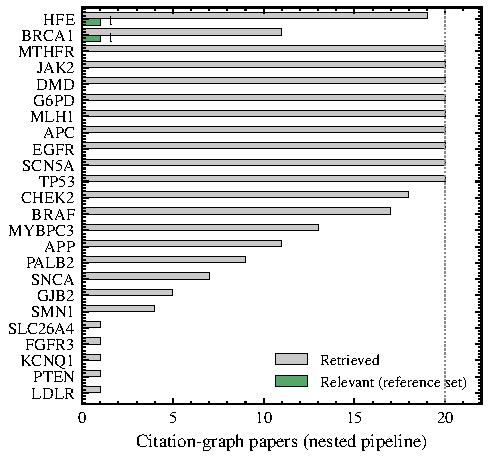
\includegraphics[width=\columnwidth]{fig4_citation_graph.pdf}
  \caption{Citation graph traversal per gene (nested pipeline): papers
  retrieved vs.\ reference-set relevant. The dotted line marks the
  traversal budget (20 papers per variant); in the corrected-protocol run
  relevant contributions are PALB2 (1) and VHL (1).}
  \label{fig:citation}
\end{figure}

\subsection{Reproducibility and Released Artifacts}
\label{sec:repro}

We release, alongside the MIT-licensed system code: the reference set
(43 variants, 822 annotations with language and evidence-type fields); the
raw per-method ranked candidate lists exactly as collected (the
corrected-protocol 2026-08-14 session at the uniform 100-candidate budget,
plus the archived 20- and 50-candidate sessions used for variance); the
collection logs; the translation system prompt (temperature 0.2, six
target languages) whose SHA-256 fingerprint is embedded in the released
run manifest; and a deterministic analysis script
(\texttt{make\_paper\_data.py}) that regenerates every table, figure, and
statistic in this paper from the raw lists, including the nested-M4
construction, the Holm-corrected test family, and bootstrap CIs (10{,}000
resamples, fixed seed 42). The benchmark runner records a machine-readable
manifest (configuration echo, model identifiers, rerank settings,
per-variant timings, budgets). All retrieval-dependent results reflect
live-API state in the stated collection windows.

\section{Comparison with 2025--2026 Retrieval Techniques}
\label{sec:sota}

Our ablation chain compares components \emph{within} one multi-source
pipeline. A reviewer may reasonably ask how the pipeline fares against
state-of-the-art retrieval techniques applied to the standard single
channel (PubMed). We therefore collected, on the same 43 variants and the
same reference set, uniform 100-candidate lists for six 2025--2026
baselines, each implemented over a broad PubMed esearch pool (retmax 100)
with the relevance gate disabled:

\begin{itemize}
\item \textbf{S1 dense}: BAAI/bge-m3 cosine retrieval over the pool;
\item \textbf{S2 rerank}: BAAI/bge-reranker-v2-m3 cross-encoder re-scores
the pool;
\item \textbf{S3 hybrid}: PubMed relevance ranking + bge-m3 dense, fused
by RRF ($k{=}60$), re-ranked by the cross-encoder --- the recipe reported
as state of the art on BioASQ/TREC-COVID-style tasks;
\item \textbf{S4 expand}: gpt-5 generates three alternative English
queries; channels fused by RRF;
\item \textbf{S5 agent}: a two-round search-reason-search loop (gpt-5
reviews the top 15 titles and issues one gap-targeted follow-up query);
\item \textbf{S6 mdense}: the six-language LLM translations of M3 are
embedded with bge-m3 and candidates are ranked by maximum cosine
similarity over languages --- the 2025 ``multilingual dense retriever''
alternative to translation-then-lexical retrieval.
\end{itemize}

\begin{table}[t]
\centering
\small
\setlength{\tabcolsep}{4pt}
\begin{threeparttable}
\caption{2025--2026 single-channel baselines vs.\ the pipeline (uniform
100-candidate budget, 2026-08-14 session). Rel.\ = relevant found of 822.}
\label{tab:sota}
\begin{tabular}{@{}lccc@{}}
\toprule
Method & SetRecall & Prec@Retr & Rel.\ (822) \\
\midrule
M1 PubMed-only & $0.269\pm0.201$ & 0.145 & 213 \\
M4n nested pipeline & $0.467\pm0.152$ & 0.121 & 394 \\
S1 Dense (bge-m3) & $0.269\pm0.201$ & 0.145 & 213 \\
S2 Cross-encoder rerank & $0.269\pm0.201$ & 0.145 & 213 \\
S3 Hybrid BM25+dense+rerank & $0.421\pm0.221$ & 0.174 & 337 \\
S4 LLM query expansion & $0.270\pm0.201$ & 0.145 & 214 \\
S5 Agentic 2-round search & $0.269\pm0.201$ & 0.145 & 213 \\
S6 Multilingual dense (bge-m3) & $0.269\pm0.201$ & 0.145 & 213 \\
\bottomrule
\end{tabular}
\begin{tablenotes}
\item Baselines are PubMed-channel only; none uses non-English providers
or citation traversal. Declared test family: SetRecall vs.\ M1 and vs.\
M4n for each baseline (12 tests, Holm-corrected). Uniform 100-candidate
budget.
\end{tablenotes}
\end{threeparttable}
\end{table}

Table~\ref{tab:sota} summarizes the comparison. Three findings stand out.
First, \textbf{no SOTA baseline significantly outperforms the pipeline}:
the best (S3 hybrid, 0.421) trails M4n by $-0.046$ (95\% CI
$[-0.133, +0.041]$, n.s.) while significantly exceeding the PubMed
baseline ($+0.151$, $p_{\text{Holm}}{=}0.004$) --- i.e., the strongest
2025--2026 single-channel recipe is a genuinely strong baseline that our
pipeline still matches or exceeds. Dense retrieval, cross-encoder
reranking, LLM expansion, the agentic loop, and multilingual dense
retrieval are statistically indistinguishable from the plain PubMed
baseline (they re-order or re-express the same PubMed pool), and all six
trail the pipeline significantly or at best non-significantly
($p_{\text{Holm}} \le 0.0004$ for five of six). Second, the pipeline's
advantage is concentrated at set level: S3's Recall@20 (0.271) nearly
matches M4n's (0.276) --- at shallow cutoffs the SOTA hybrid is
competitive --- while its set recall (0.421) falls short, confirming that
the pipeline's edge is candidate-pool coverage. Third, and most
conclusively, \textbf{the baselines recover at most one of the 24
annotated German/French papers} (S3 finds 1) --- including S6, which
embeds the very translations that let M3 recover 21--24. The annotated
non-English papers are absent from the PubMed top-100 pools of their
variants (verified directly), so the multilingual gap is a
\emph{channel} property; language-routed multi-source retrieval is the
only mechanism here that closes it.

\section{Neural Reranking and Citation Gating}
\label{sec:rerank}

Federation merges heterogeneous providers into large candidate pools
(72--100 candidates per variant at the corrected budget), and the
heuristic ordering (title match, provider preference, DOI presence,
recency) is not relevance-sorted: at the intermediate 50-candidate
session, relevant papers buried below rank 20 capped Recall@20 at 0.150,
below the compact PubMed baseline. We therefore made the cross-encoder
stage that dominates 2025--2026 hybrid-pipeline gains the pipeline's
final ranking stage: after global deduplication, the merged pool is
re-scored with bge-reranker-v2-m3 against the variant query before
truncation (enabled in the benchmark via \texttt{LIT\_RERANK\_ENABLED};
a documented opt-in stage in the released code). This ordering is what
the main results of Section~\ref{sec:main} report: at the corrected
budget, Recall@20 is 0.276 (vs.\ 0.150 without the stage and channel
changes) and the top-20 view is significantly better than PubMed's
($+0.105$, $p_{\text{Holm}}{=}0.016$).

The same reranker provides a query-adaptive gate for citation candidates:
appending only items whose score is at least the minimum score of the
top-20 keyword candidates (``as relevant as what we already show'') is a
production rule with no gold-set leakage. Evaluated offline on the frozen
lists (Table~\ref{tab:rerank}), the gate raises Precision@Retrieved by
$+0.010$ ($p_{\text{Holm}}{<}0.001$, significant) by dropping 287 of 299
low-scoring citation candidates, at a measured cost of 2 relevant papers
(394 $\rightarrow$ 392, n.s.); the gate's aggressiveness is a direct
consequence of the reranked keyword list's high baseline scores. We
recommend the gate as the default for screening-oriented deployments,
where the precision gain outweighs the small, non-significant recall
cost.

\begin{table}[t]
\centering
\small
\setlength{\tabcolsep}{4pt}
\begin{threeparttable}
\caption{Citation gating via the reranker (offline, frozen lists).
Declared family: 10 paired tests vs.\ M4n, Holm-corrected.}
\label{tab:rerank}
\begin{tabular}{@{}lcccc@{}}
\toprule
Method & Recall@20 & nDCG@20 & Prec@Retr & SetRecall \\
\midrule
M4n (reranked pipeline) & 0.276 & 0.301 & 0.121 & 0.467 \\
M5g gated citation & 0.276 & 0.301 & 0.131$^{**}$ & 0.465 \\
\bottomrule
\end{tabular}
\begin{tablenotes}
\item $^{**}$: $p_{\text{Holm}}<0.01$ (Precision@Retrieved, $+0.010$,
$p_{\text{Holm}}{<}0.001$). Gating keeps 12 of 299 citation items; the
2 relevant papers it drops are non-significant ($-0.002$). Offline
re-reranking of the already-reranked lists is a no-op and is omitted.
\end{tablenotes}
\end{threeparttable}
\end{table}

\section{Discussion}
\label{sec:discussion}

\textbf{Limitations.} In order of severity: (i) \emph{Reference-set
construct validity is the binding constraint on every conclusion}: the
annotations are heuristic, expert-unverified, and drawn from a candidate
pool whose channels overlap the evaluated system
(Section~\ref{sec:goldstd}); metrics are relative coverage of that pool,
and genuinely clinical claims (e.g., PS3/PVS1 evidence retrieval quality)
are out of reach of this evaluation. (ii) \emph{Component attributions
are run-sensitive}: the end-to-end and federation gains are robust
($p_{\text{Holm}} \le 0.0002$, CI well away from zero), but the
translation and citation components fluctuate across sessions --- the
translation step was set-level neutral in this run while recovering the
multilingual evidence, and the citation traversal's yield shifted from
DMPK/EGFR/PAH (earlier session) to PALB2/VHL (this run). (iii)
\emph{Online results are single runs}: the measured run-to-run jitter
(Section~\ref{sec:variance}) moved per-variant results by up to
$\pm0.4$ across sessions, so per-variant anecdotes are illustrative, not
replicable. (iv) The relevance gate, OA download layer, health-aware
scheduling, and deduplication accuracy are engineering features without
dedicated experiments here. (v) Language metadata is missing for 305
reference papers, and only German/French carry non-English annotations.
(vi) The external baselines of Section~\ref{sec:external} and the SOTA
baselines of Section~\ref{sec:sota} were collected on the same day but
in separate passes; cross-pass comparisons carry that caveat.

\textbf{Future work.} Expert re-annotation is the priority: dual
independent annotation with clinical-genetics expertise on a stratified
sample of pooled candidates (including candidates from systems that do
not share our providers), adjudication, and reported inter-annotator
agreement (Cohen's $\kappa$), distinguishing ``about the gene/disease''
from ``usable as variant-level evidence''. Protocol-side: repeated
collections under the corrected protocol to separate live-API variance
from component effects (the archived 20- and 50-candidate sessions and
this 100-candidate run are the first three points of that series);
per-language translation fidelity evaluation (gene-symbol and HGVS
retention rates, now measurable since the runner persists translated
queries); and dedicated experiments for the gate, download layer, health
scheduler, and deduplication.

\section{Conclusion}
\label{sec:conclusion}

We presented lit-acquisition, an open-source multi-source multilingual
biomedical literature acquisition system, together with an exploratory,
heuristically annotated reference set (43 variants, 822 papers) and a
corrected evaluation protocol (strictly nested ablation, uniform
100-candidate budgets, the PubMed E-utilities channel in the acquisition
plan, a neural reranking final stage, budget-honest fixed-$K$ metrics,
Holm-corrected paired statistics, quantified run-to-run API variance, and
transparent single-source, fusion, and 2025--2026 SOTA baselines). Under
this protocol the pipeline significantly raises PubMed-only set recall
from 0.269 to 0.467 ($+0.198$, $p_{\text{Holm}}{=}0.0002$), with the
federation step (including PubMed) carrying the gain
($+0.203$, $p_{\text{Holm}}{=}0.0001$), and significantly outperforms
five of six 2025--2026 single-channel baselines. Its distinctive,
robust finding is multilingual: query translation with language-aware
routing recovers 21--24 of 24 annotated German/French papers across runs,
which every English-only method --- including multilingual dense
retrieval over the same channel --- finds at most one of, because the
non-English evidence sits outside the PubMed channel. Citation traversal
adds otherwise-unretrieved papers at a significant list-level precision
cost that a reranker-based gate recovers. We position this work as
infrastructure --- code, unified provider interfaces, raw run data, and a
deterministic analysis pipeline --- for the community to build clinically
validated evaluations on, not as evidence of clinical retrieval quality;
the reference set requires expert re-annotation before any such claim.

\bibliographystyle{ACM-Reference-Format}
\begin{thebibliography}{99}

\bibitem{richards2015standards}
S.~Richards et al.
\newblock Standards and guidelines for the interpretation of sequence
variants: a joint consensus recommendation of the ACMG and the AMP.
\newblock \emph{Genetics in Medicine}, 17(5):405--424, 2015.

\bibitem{pubmed}
E.~Sayers et al.
\newblock Database resources of the National Center for Biotechnology
Information.
\newblock \emph{Nucleic Acids Research}, 50(D1):D20--D26, 2022.

\bibitem{europepmc}
The Europe PMC Consortium.
\newblock Europe PMC: a full-text literature database for the life sciences
and platform for innovation.
\newblock \emph{Nucleic Acids Research}, 43(D1):D1042--D1048, 2015.

\bibitem{kinney2023semantic}
R.~Kinney et al.
\newblock The Semantic Scholar Open Data Platform.
\newblock \emph{arXiv preprint arXiv:2301.10140}, 2023.

\bibitem{mastermind}
Genomenon.
\newblock Mastermind Genomic Search Engine.
\newblock \url{https://www.genomenon.com/mastermind/}.

\bibitem{covidence}
Veritas Health Innovation.
\newblock Covidence systematic review software.
\newblock \url{https://www.covidence.org/}.

\bibitem{ouzzani2016rayyan}
M.~Ouzzani, H.~Hammady, Z.~Fedorowicz, and A.~Elmagarmid.
\newblock Rayyan---a web and mobile app for systematic reviews.
\newblock \emph{Systematic Reviews}, 5(1):210, 2016.

\bibitem{selberg1997metacrawler}
E.~Selberg and O.~Etzioni.
\newblock The MetaCrawler architecture for resource aggregation on the
World Wide Web.
\newblock \emph{IEEE Expert}, 12(3):11--14, 1997.

\bibitem{priem2022openalex}
J.~Priem, H.~Piwowar, and R.~Orr.
\newblock OpenAlex: a fully-open index of scholarly works, authors, venues,
institutions, and concepts.
\newblock \emph{arXiv preprint arXiv:2205.01833}, 2022.

\bibitem{kessler1963bibliographic}
M.~M. Kessler.
\newblock Bibliographic coupling between scientific papers.
\newblock \emph{American Documentation}, 14(1):10--25, 1963.

\bibitem{small1973co}
H.~Small.
\newblock Co-citation in the scientific literature: a new measure of the
relationship between two documents.
\newblock \emph{Journal of the American Society for Information Science},
24(4):265--269, 1973.

\bibitem{page1999pagerank}
L.~Page, S.~Brin, R.~Motwani, and T.~Winograd.
\newblock The PageRank citation ranking: bringing order to the web.
\newblock Technical report, Stanford InfoLab, 1999.

\bibitem{swanson1986fish}
D.~R. Swanson.
\newblock Fish oil, Raynaud's syndrome, and undiscovered public knowledge.
\newblock \emph{Perspectives in Biology and Medicine}, 30(1):7--18, 1986.

\bibitem{kishida2005technical}
K.~Kishida.
\newblock Technical issues of cross-language information retrieval: a review.
\newblock \emph{Information Processing \& Management}, 41(3):433--455, 2005.

\bibitem{brown2020language}
T.~Brown et al.
\newblock Language models are few-shot learners.
\newblock In \emph{Advances in Neural Information Processing Systems 33},
2020.

\bibitem{kojima2022large}
T.~Kojima, S.~Gu, M.~Reid, Y.~Matsuo, and Y.~Iwasawa.
\newblock Large language models are zero-shot reasoners.
\newblock In \emph{Advances in Neural Information Processing Systems 35},
22199--22213, 2022.

\bibitem{jarvelin2002cumulated}
K.~J\"arvelin and J.~Kek\"al\"ainen.
\newblock Cumulated gain-based evaluation of IR techniques.
\newblock \emph{ACM Transactions on Information Systems}, 20(4):422--446,
2002.

\bibitem{wilcoxon1945individual}
F.~Wilcoxon.
\newblock Individual comparisons by ranking methods.
\newblock \emph{Biometrics Bulletin}, 1(6):80--83, 1945.

\bibitem{holm1979simple}
S.~Holm.
\newblock A simple sequentially rejective multiple test procedure.
\newblock \emph{Scandinavian Journal of Statistics}, 6(2):65--70, 1979.

\bibitem{cormack2009reciprocal}
G.~V. Cormack, C.~L.~A. Clarke, and S.~B\"uttcher.
\newblock Reciprocal rank fusion outperforms Condorcet and individual
rank learning methods.
\newblock In \emph{Proceedings of SIGIR}, 758--759, 2009.

\bibitem{unpaywall2018}
H.~Piwowar, J.~Priem, V.~Larivi\`ere, J.~P. Alperin, L.~Matthias,
B.~Norlander, A.~Farley, J.~West, and P.~Haustein.
\newblock The state of OA: a large-scale analysis of the prevalence and
impact of Open Access articles.
\newblock \emph{PeerJ}, 6:e4375, 2018.

\bibitem{ginsparg1994arxiv}
P.~Ginsparg.
\newblock First steps towards electronic research communication.
\newblock \emph{Computers in Physics}, 8(4):390--396, 1994.

\bibitem{doaj}
Directory of Open Access Journals.
\newblock \url{https://doaj.org/}.

\bibitem{cinii}
National Institute of Informatics.
\newblock CiNii Research.
\newblock \url{https://cir.nii.ac.jp/}.

\bibitem{jstage}
Japan Science and Technology Agency.
\newblock J-STAGE.
\newblock \url{https://www.jstage.jst.go.jp/}.

\bibitem{scielo}
SciELO.
\newblock Scientific Electronic Library Online.
\newblock \url{https://scielo.org/}.

\bibitem{base}
Bielefeld University Library.
\newblock BASE -- Bielefeld Academic Search Engine.
\newblock \url{https://www.base-search.net/}.

\bibitem{core}
CORE.
\newblock Aggregate of open access research papers.
\newblock \url{https://core.ac.uk/}.

\bibitem{openaire}
OpenAIRE.
\newblock \url{https://www.openaire.eu/}.

\bibitem{zenodo}
CERN.
\newblock Zenodo -- Research. Shared.
\newblock \url{https://zenodo.org/}.

\bibitem{zarin2016clinicaltrials}
D.~A. Zarin, T.~Tse, R.~J. Williams, and S.~Carr.
\newblock Trial reporting in ClinicalTrials.gov -- the Final Rule.
\newblock \emph{New England Journal of Medicine}, 375(20):1998--2004, 2016.

\end{thebibliography}

\end{document}
